\subsection{Giới thiệu về bài toán Object Detection}
Trong phần này nhóm sẽ giới thiệu về thị giác máy tính (Computer Vision – CV) và bài toán Object Detection \cite{objectdetection}.

Thị giác máy tính có thể giải thích đơn giản như sau: Đó là một lĩnh vực của trí tuệ nhân tạo (AI) và khoa học máy tính liên quan đến việc xử lý, phân tích và hiểu các hình ảnh và video. Nó tập trung vào việc tạo ra các thuật toán và phương pháp để cho máy tính có khả năng nhìn và hiểu thế giới xung quanh giống như con người bình thường.

Một số bài toán trong lĩnh vực này bao gồm Image classification, Classification with Localization, Object Detection, Instance Segmentation.

\graphicspath{{figures/}}
\begin{figure}[h!]
  \centering
  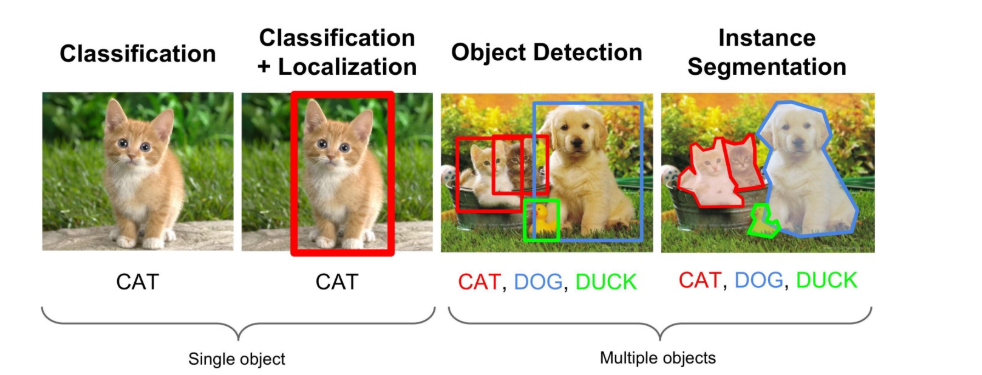
\includegraphics[scale=0.4]{graphics/Hinh1.png}
  \caption{Một số bài toán trong lĩnh vực CV}
\end{figure}

% \begin{center}
%     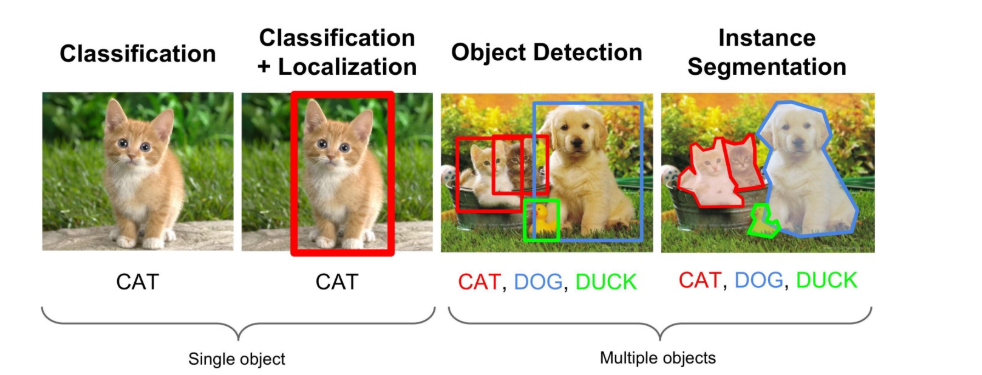
\includegraphics[scale=0.45]{graphics/Hinh1.png}
% \end{center}

\graphicspath{{figures/}}
\begin{figure}[h!]
  \centering
  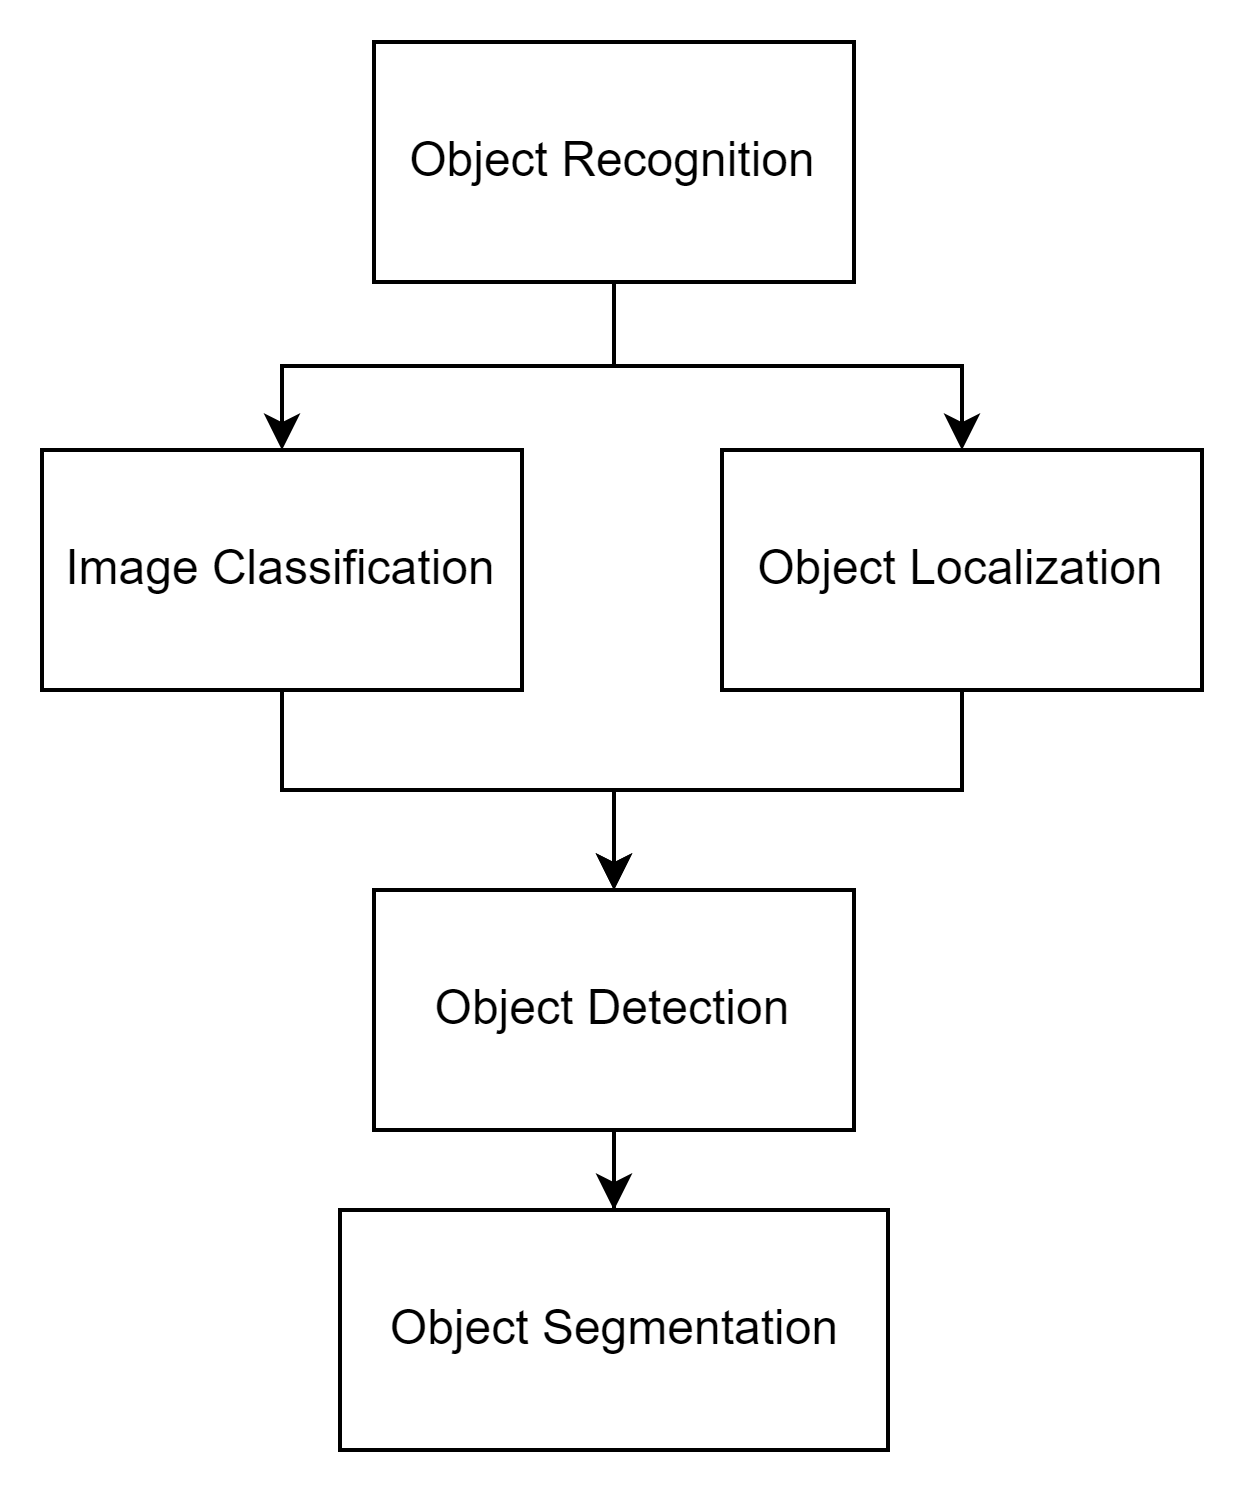
\includegraphics[scale=0.18]{graphics/general.png}
  \caption{Sơ lược mối liên hệ giữa các tác vụ trong thị giác máy tính}
\end{figure}
Trong lĩnh vực Thị giác máy tính và Trí tuệ nhân tạo, bài toán Object Detection đã trở thành một chủ đề quan trọng và hấp dẫn. Bài toán này đóng vai trò cốt lõi trong việc xác định và định vị các đối tượng trong một hình ảnh hoặc video. Hiểu và giải quyết bài toán này mang lại nhiều ứng dụng thực tế, như trong lĩnh vực tự lái xe, giám sát an ninh, phân loại hình ảnh và nhận dạng khuôn mặt.

Bài toán Object Detection (nhận diện vật thể) trong đó mục tiêu là xác định và phân loại các vật thể xuất hiện trong hình ảnh hoặc video. Bài toán này đòi hỏi mô hình máy tính phải có khả năng phát hiện và định vị vật thể trong hình ảnh, đồng thời gán nhãn cho chúng thuộc các lớp vật thể khác nhau. Ta phải đối mặt với các thách thức như sự biến đổi về kích thước, hình dạng và góc nhìn của vật thể, đồng thời còn phải xử lý các vấn đề như nhiễu, che khuất và độ phức tạp của môi trường.

\graphicspath{{figures/}}
\begin{figure}[h!]
  \centering
  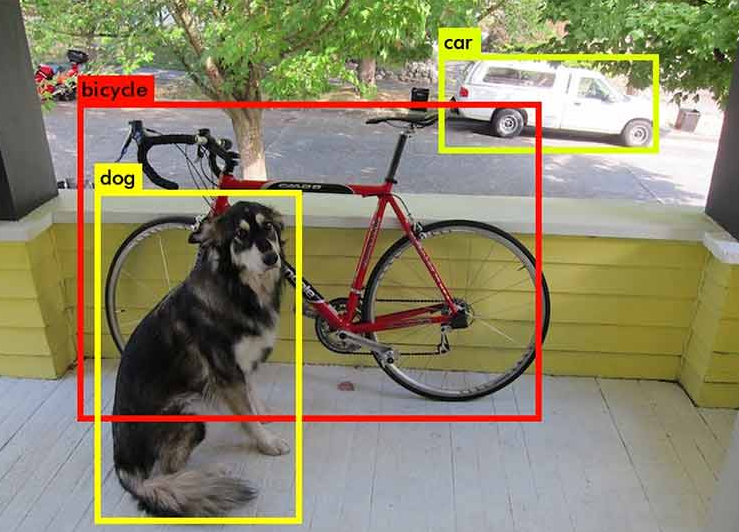
\includegraphics[scale=0.4]{graphics/object detection.png}
  \caption{Ví dụ về bài toán Object Detection}
\end{figure}

Một số phương pháp truyền thống đã được sử dụng cho bài toán Object Detection bao gồm phân đoạn ảnh, phát hiện biên, phương pháp dựa trên cửa sổ trượt và phương pháp dựa trên các đặc trưng cục bộ. Mặc dù các phương pháp này có những ưu điểm riêng, nhưng chúng cũng gặp phải một số hạn chế, đặc biệt là khi xử lý các hình ảnh có nhiều đối tượng và độ phức tạp cao.

Với sự phát triển của Deep Learning, các mô hình dựa trên mạng neural đã mang lại những bước tiến đáng kể trong việc giải quyết bài toán Object Detection, kể đến như R-CNN, Fast R-CNN, Faster R-CNN và YOLO. Những mô hình này sử dụng các kiến trúc mạng neural phức tạp để xác định và định vị các đối tượng một cách hiệu quả trong hình ảnh.

Ứng dụng của Object Detection rất đa dạng và phong phú. Trong lĩnh vực tự lái xe, Object Detection được sử dụng để phát hiện và phản ứng với các đối tượng như xe, người đi bộ, biển báo giao thông và điều kiện đường. Trong giám sát an ninh, nó có thể giúp xác định và theo dõi các đối tượng đáng ngờ trong các hình ảnh hoặc video giám sát. Bên cạnh đó, Object Detection cũng có thể áp dụng trong các lĩnh vực như phân loại hình ảnh và nhận dạng khuôn mặt.

\graphicspath{{figures/}}
\begin{figure}[h!]
  \centering
  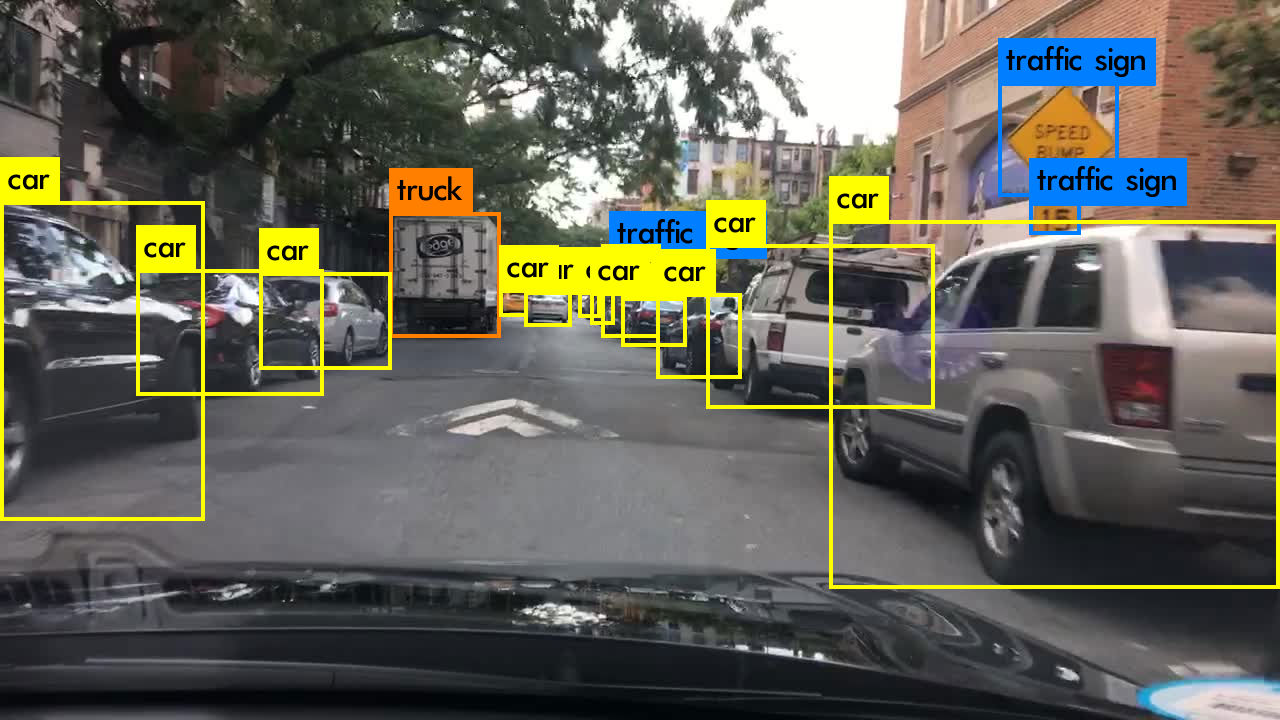
\includegraphics[scale=0.3]{graphics/Object Detection in Autonomous Driving.jpg}
  \caption{Object Detection ứng dụng trong xe tự hành}
\end{figure}

Với những tiến bộ trong Deep Learning và sự phát triển của công nghệ, bài toán Object Detection đang trở thành một lĩnh vực nghiên cứu hứa hẹn. Việc nghiên cứu và áp dụng những phương pháp hiện đại trong bài toán này có thể mang lại những ứng dụng thực tiễn mạnh mẽ trong tương lai.

\subsection{Giới thiệu về đồ án}
Đồ án này tập trung vào bài toán Pedestrian Detection, một đề tài không còn quá xa lạ đối với những người đã và đang tiếp cận bài toán Object Detection. Bài toán này nhằm xác định và định vị vị trí của người đi bộ trong các hình ảnh hoặc video, có ứng dụng rộng rãi trong nhiều lĩnh vực như giám sát an ninh, xe tự hành và các hệ thống nhận diện. Đồ án sẽ trình bày hai cách tiếp cận khác nhau để giải quyết bài toán Pedestrian Detection, đó là sử dụng mô hình HOG+SVM và mô hình Faster R-CNN.

\graphicspath{{figures/}}
\begin{figure}[h!]
  \centering
  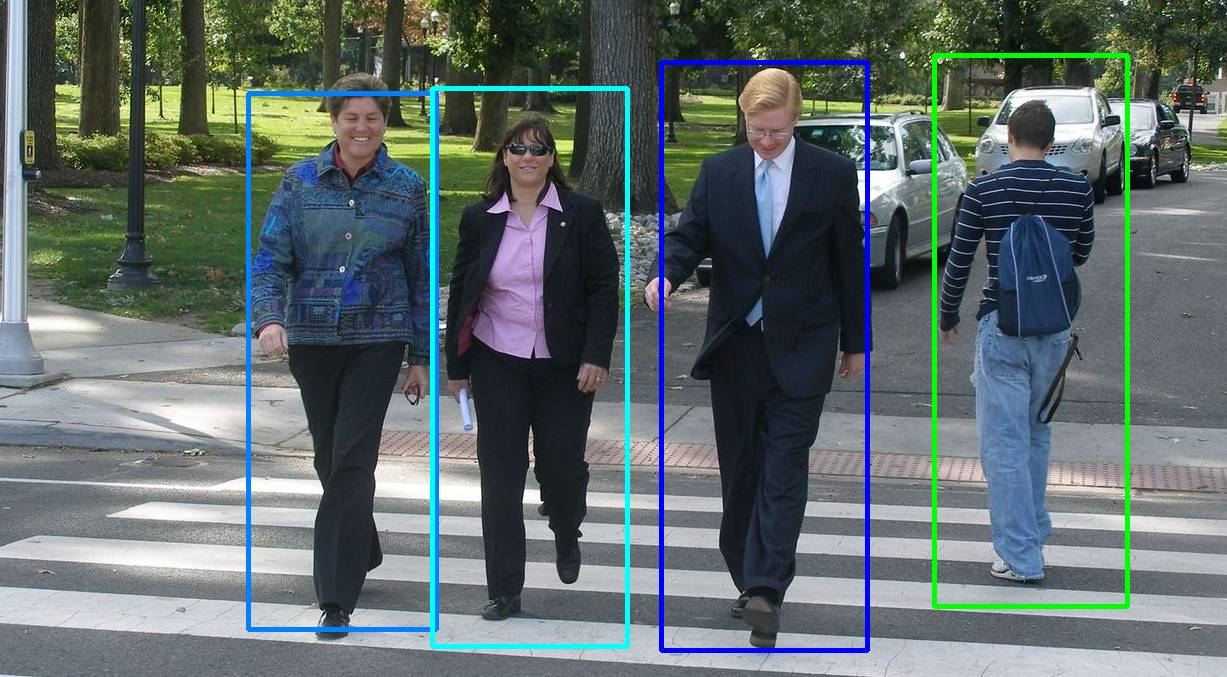
\includegraphics[scale=0.39]{graphics/Hinh2.jpg}
  \caption{Nhận diện người đi bộ (Pedestrian Detection)}
\end{figure}

Cách tiếp cận đầu tiên của nhóm sẽ sử dụng mô hình HOG (Histogram of Oriented Gradients) kết hợp với SVM (Support Vector Machine). Mô hình HOG là một phương pháp biểu diễn đặc trưng được sử dụng để mô tả hình dạng của đối tượng. Bằng cách tính toán gradient của các khối hình ảnh, HOG tạo ra một biểu diễn đặc trưng mô tả sự phân bố các đường cạnh và hướng của hình ảnh. Sau đó, SVM được sử dụng để phân loại đối tượng có chứa người đi bộ hoặc không. Mô hình HOG+SVM đã được chứng minh là hiệu quả trong việc phát hiện người đi bộ trong ảnh tĩnh.

Cách tiếp cận thứ hai sẽ sử dụng mô hình Faster R-CNN (Region-based Convolutional Neural Network). Mô hình này kết hợp giữa hai thành phần chính là mạng neural tích chập (CNN) và mạng neural nhận diện vùng đặc trưng (R-CNN). Với Faster R-CNN, đầu tiên, một mạng CNN được sử dụng để trích xuất các đặc trưng từ hình ảnh. Sau đó, mạng R-CNN được sử dụng để phát hiện và định vị vùng chứa người đi bộ dựa trên các đặc trưng đã trích xuất. Mô hình Faster R-CNN có khả năng tự động học các đặc trưng phù hợp với bài toán Pedestrian Detection, đồng thời cung cấp độ chính xác cao.

Trong quá trình thực hiện đồ án, nhóm sẽ tiến hành huấn luyện và đánh giá hiệu suất của cả hai cách tiếp cận trên tập dữ liệu đã được gán nhãn, chứa các hình ảnh có chứa và không chứa người đi bộ. Hiệu suất của các mô hình sẽ được đánh giá dựa trên độ đo mAP.

\subsection{Lý do chọn đề tài}
Đề tài này được nhóm chọn dựa trên sự quan tâm từ việc ứng dụng nhận dạng đối tượng có thể mang lại trong các lĩnh vực như an ninh, xử lý ảnh, và tự động hóa công nghiệp. Mục tiêu của đồ án nhận diện người đi bộ này là phân loại và xác định vị trí chính xác của các người đi bộ trong hình ảnh để tạo nền tảng cho việc xây dựng các ứng dụng thông minh dựa trên thị giác máy tính.

Một ứng dụng cho bài toán nhận diện người đi bộ vô cùng thực tế mà nhóm đã được thầy góp ý là việc ứng dụng nó trong các siêu thị, trung tâm thương mại để quan sát vị trí nào mà khách hàng tập trung nhiều nhất để từ đó đưa ra các biện pháp tối ưu hóa trải nghiệm mua sắm và cải thiện quản lý cửa hàng. Bằng cách sử dụng hệ thống nhận diện người đi bộ, siêu thị và trung tâm thương mại có thể phân tích và đếm số lượng khách hàng tại các khu vực khác nhau trong cửa hàng. Thông qua việc phân tích dữ liệu, họ có thể xác định vị trí nào thu hút nhiều khách hàng nhất và tạo ra các chiến lược trưng bày sản phẩm hiệu quả để tăng doanh số bán hàng.
\pagebreak
\begin{figure}[h!]
  \centering
  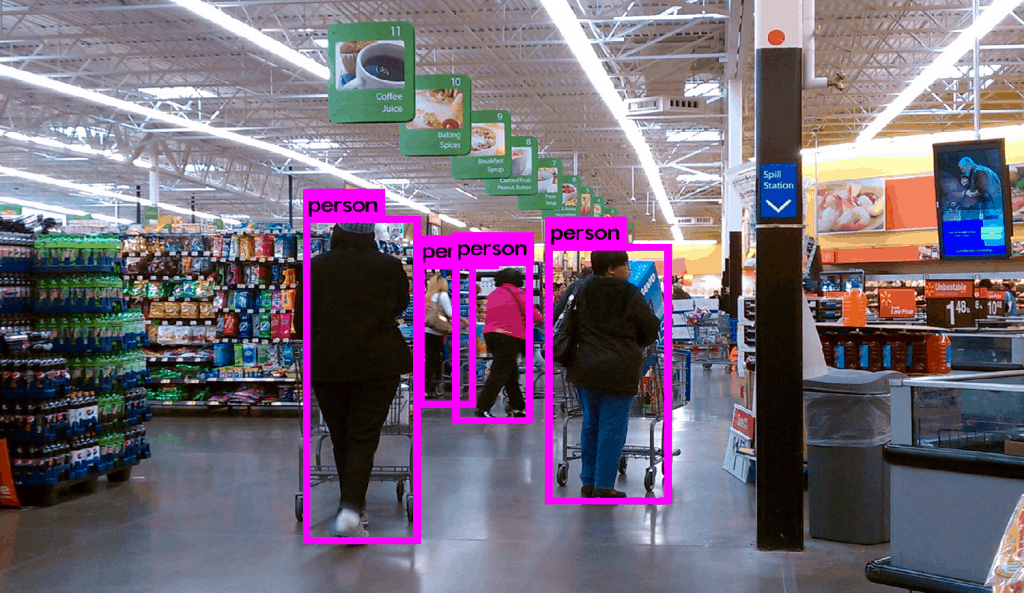
\includegraphics[scale=0.3]{graphics/supermarket.png}
  \caption{Nhận diện người đi bộ trong siêu thị}
\end{figure}

Để đạt được mục tiêu nghiên cứu, nhóm đã lựa chọn hai phương pháp để thực hiện: HOG+SVM và Faster R-CNN.

%Phương pháp HOG+SVM (Histogram of Oriented Gradients và Support Vector Machine) đã được nhóm chọn để thực nghiệm vì tính đơn giản và hiệu quả trong nhận dạng đối tượng. HOG giúp trích xuất đặc trưng từ hình ảnh bằng cách tính toán histogram các hướng cạnh trong hình ảnh. Sau đó, SVM được sử dụng để huấn luyện mô hình phân loại dựa trên các đặc trưng HOG trích xuất từ hình ảnh. Sự kết hợp của HOG và SVM cho phép chúng ta xây dựng một hệ thống nhận dạng đối tượng đơn giản và có hiệu suất tốt trong một số trường hợp.

%Ngoài ra, nhóm cũng đã chọn phương pháp Faster R-CNN (Region-based Convolutional Neural Network) để thực nghiệm do khả năng kết hợp giữa việc phân loại đối tượng và định vị vị trí chính xác của chúng. Faster R-CNN sử dụng mạng neural convolutional để trích xuất đặc trưng từ hình ảnh và sau đó sử dụng một mạng neural định vị để xác định vùng chứa các đối tượng trong hình ảnh. Phương pháp này cho phép chúng ta đạt được hiệu suất cao trong việc phát hiện và phân loại các đối tượng trong hình ảnh, đồng thời cung cấp vị trí chính xác của từng đối tượng.

%Lựa chọn hai phương pháp HOG+SVM và Faster R-CNN cho bài toán này đảm bảo một phạm vi rộng hơn trong việc so sánh và đánh giá hiệu suất của các phương pháp nhận dạng đối tượng khác nhau. Điều này giúp tăng cường kiến thức và sự hiểu biết về cách thức hoạt động và ưu điểm của từng phương pháp, từ đó đưa ra kết luận và đề xuất cho việc áp dụng trong các ứng dụng thực tế.
Việc lựa chọn hai phương pháp này xuất phát từ sự tò mò và mong muốn học hỏi thêm kiến thức về lĩnh vực thị giác máy tính. Chúng em muốn khám phá và so sánh sự khác biệt giữa các phương pháp machine learning và deep learning để hiểu rõ hơn về cách thức hoạt động và ưu điểm của từng phương pháp. Từ việc nghiên cứu này, nhóm chúng em đã được trau dồi kiến thức và hiểu biết sâu hơn về lĩnh vực đang học.